\newpage % Rozdziały zaczynamy od nowej strony.
\section{Wyniki pracy}
Niniejszy rozdział prezentuje główne wyniki uzyskane w trakcie badania i zawiera w sobie podsumowanie przeprowadzonych eksperymentów. Omówione zostaną w nim wszystkie uzyskane rezultaty, które pozwalają na ocenę czy sztuczne sieci neuronowe mogą być stosowane z powodzeniem w obszarze regulacji. Na początku zaprezentowany zostanie sposób generacji danych, poczynione założenia i sposób działania regulacji opartej o sieć neuronową. Kolejno wybrana zostanie optymalna liczba neuronów warstwy ukrytej pozwalająca na minimalizację funkcji celu z zachowaniem ogólności rozwiązania. W kolejnej części zbadany zostanie wpływ zastosowania redukcji sieci na osiągane przez nią rezultaty. Po wybraniu optymalnej struktury i pełnym wytrenowaniu sieci zbadamy jak poradzi sobie z regulacją obiektów, które nie znalazły odzwierciedlenia w przykładach uczących. Ciekawym eksperymentem będzie też sprawdzenie działania sieci w przypadku wielokrotnych skoków wartości zadanej. Pod koniec rozdziału sformułowane zostaną ogólne wnioski i uwagi płynące z całości eksperymentów, które znajdą również swoje odzwierciedlenie w późniejszym podsumowaniu pracy.

\subsection{Generacja danych}
Niezbędnym krokiem przed przystąpieniem do trenowania sieci neuronowej jest generacja danych, na podstawie których sieć następnie zostanie nauczona. Celem pracy jest zweryfikowanie zdolności adaptacji sieci do działania jako regulator DMC. Kierując się tym założeniem oczywistym wydaje się wygenerowanie danych uczących na podstawie symulacji przeprowadzonych z wykorzystaniem rzeczywistego regulatora DMC. Praca ma jedynie charakter porównawczy, a więc za najogólniejszy przykład regulacji możemy wybrać dostosowanie wyjścia obiektu regulacji do jednokrotnego skoku wartości zadanej. Jako obiekt regulacji wybrany został w tej części układ opisany we wcześniejszej części pracy, który identyfikujemy poprzez następujące parametry: \( T_1=5, \, T_2=2, \, K=1, \, T_d=0 \). Wybór dokonany został w sposób arbitralny, gdyż przeprowadzenie eksperymentów z wykorzystaniem dowolnego innego układu pozwala osiągnąć zbliżone rezultaty i wyciągnąć analogiczne wnioski.
\par Na tym etapie należy podjąć decyzję odnośnie wartości na podstawie, których sieć neuronowa dokonywać będzie regulacji. Kierując się analogią do klasycznych metod za dobrą metodę wybrano sterowanie na podstawie wartości uchybu regulacji oraz aktualnej wartości zadanej. W trakcie przeprowadzanych eksperymentów długość symulacji wynosi 40 okresów jako okres, po którym układ regulowany za pomocą regulatora DMC osiąga pełną stabilność. Na tej podstawie do sterowania za pomocą sieci wybrane zostało 30 wartości uchyby regulacji oraz aktualna wartość zadana. Wyjściem sieci jest oczywiście pojedynczy sygnał sterujący co stanowi pewną modyfikację względem algorytmu DMC gdzie, w każdej iteracji wyznaczana jest zmiana sterowania. Opisana modyfikacja stanowi jedynie szczegół implementacyjny, który nie wpływa na wyniki osiągane przez sieć.
\par Jak zostało już to opisane w części teoretycznej dane uczące i weryfikujące generowane są w sposób niezależny na podstawie oddzielnych przebiegów regulacji. Dzięki takiej strategi mamy pewność, że sieć zostanie przetestowana pod kątem ogólnej aproksymacji algorytmu OBD, a nie jedynie wybranych przebiegów regulacji. Tak więc kolejno przeprowadzone zostały eksperymenty polegające na wyznaczeniu przebiegu regulacji predykcyjnej dla jednostkowych skoków wartości zadanej z zakresu od 1 do 10 z krokiem co 0,1. Przebiegi regulacji podzielone zostały na dane uczące i weryfikujące w stosunku 75\% - 25\% . Po próbkowaniu dla każdej iteracji zbiór uczący ostatecznie składa się z 3015 przykładów, natomiast weryfikujący z 1035.
\par Ostatnim krokiem przed przystąpieniem do procedury uczenia sieci neuronowej i doboru optymalnej architektury. Jak już zostało wskazane z uwagi na sigmoidalną funkcję aktywacji koniecznym było napisanie modułu skalującego zarówno dane wejściowe jak i wyjściowe sieci do zakresu \( (-1,1 \). Warto zauważyć, że skalowanie wartości wejściowych i wyjściowych przebiega niezależnie oraz moduł skalujący umożliwia odwrotne skalowanie wartości sterowania, które następnie wykorzystywana jest w trakcie regulacji. Stanowi to istotne ograniczenie w działaniu sieci, a mianowicie sieć jest w stanie regulować tylko układy dla których pożądane wartości sterowania zawierają się w zakresie reprezentowanym przez dane wykorzystane do nauki sieci.  

\subsection{Wybór struktury sieci}
Pierwszym krokiem prowadzącym do wyselekcjonowania optymalnej architektury sieci jest wybór jej struktury. Liczba neuronów w warstwie wejściowej i wyjściowej ściśle zależy do charakterystyki problemu, a więc wygenerowanych uprzednio danych. Szczególną uwagę należy poświęcić za to prawidłowemu doborowi liczby neuronów w warstwie ukrytej. W tym celu przeprowadzono eksperyment pokazujący wartość kwadratowej funkcji kosztu w zależności od liczby neuronów w warstwie ukrytej. Przetestowano wartości z zakresu od 5 do 200 neuronów, a wyniki symulacji zaprezentowane zostały na Rysunku 5.1. 
\par Na tym etapie trenowania sieci neuronowej głównym celem jest minimalizacja funkcji kosztu na danych uczących gdyż później stosowany algorytm OBD wymaga możliwie bliskiego osiągnięcia minimum tej funkcji. W ramach przedstawienie pełniejszego obrazu na Rysunku 5.2. przedstawiona została analogiczna symulacja z wykorzystaniem danych weryfikujących (testowych). Widzimy, że wyniki obu eksperymentów są ze sobą niezwykle spójne. Obserwacja ta potwierdza intuicję, gdyż zarówno zbiór danych uczących jak i weryfikujących wygenerowany został na podstawie analogicznych symulacji, w czasie których modyfikowana była jedynie wartość zadana. 

\begin{figure}[h]
  \label{fig:Koszt-liczba-neuronow-treningowe}
  \centering 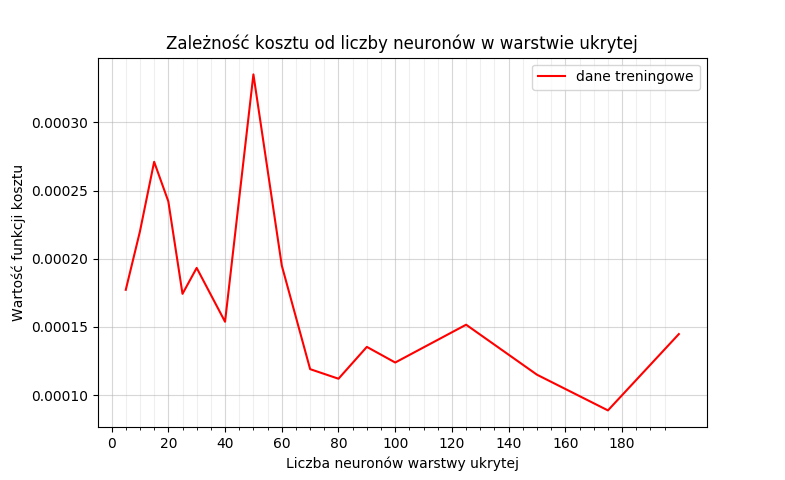
\includegraphics[width=0.7\linewidth]{cost_neuron_number_train.png}
  \caption{Zależność kosztu od liczby neuronów w warstwie ukrytej - dane treningowe}
\end{figure}

\begin{figure}[h]
  \label{fig:Koszt-liczba-neuronow-testowe}
  \centering 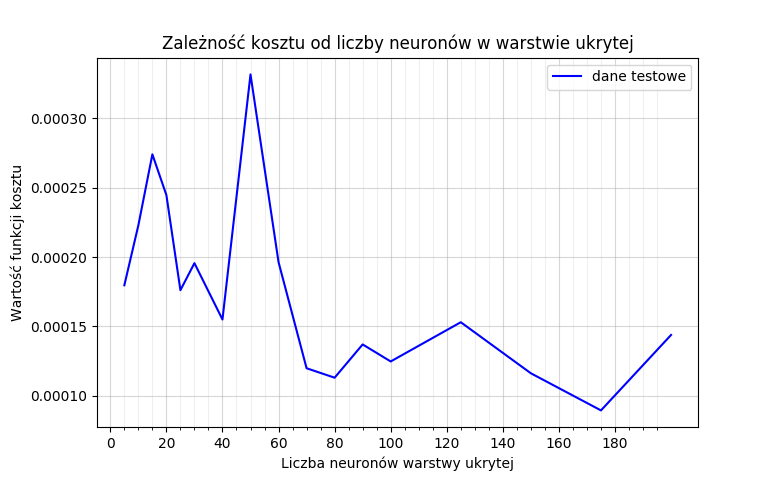
\includegraphics[width=0.7\linewidth]{cost_neuron_number_test.png}
  \caption{Zależność kosztu od liczby neuronów w warstwie ukrytej - dane testowe}
\end{figure}

\par Analiza wykresów dostarcza kilka istotnych obserwacji. Pierwszą z nich jest to, że nawet niezwykle prosta strukturą jaką jest sieć neuronowa o jedynie 5 neuronach w warstwie ukrytej jest w stanie zadowalająco dobrze nauczyć się postawionego przed nią zadania regulacji. Warto jednak zwrócić uwagę, że sieci o małej liczbie neuronów wykazują się wysoką niestabilnością przez co rezultaty przez nie osiągane mogą różnić się pomiędzy kolejnymi próbami. Po kilkukrotnym powtórzeniu eksperymentu zaobserwowano wyeliminowanie problemu dla sieci neuronowych z liczbą neuronów w warstwie ukrytych przekraczającą 100. Na tej podstawie do dalszych eksperymentów wybrana została sieć o 150 neuronach. 
\par Po wybraniu optymalnej struktury sieci należy zwrócić uwagę na zależność kosztu od liczby epok, przez które jest trenowana sieć. Pozwoli to na weryfikację wartości granicznej gradientu funkcji celu, która stanowi warunek wyjścia dla metody uczenia sieci. Początkowa kryterium wyjścia ustalone zostało na poziomie \( 10^{-5} \) co oznacza, że jeżeli gradient funkcji kosztu przez 3 kolejne iteracje jest mniejszy od zadanej wartości algorytm przerywa uczenie sieci. Eksperyment ten możemy przeprowadzić zdejmując wcześniejsze ograniczenie i sprawdzając jak zmienia się funkcja kosztu dla 300 iteracji algorytmu (epok). Wykres przedstawiający wspomnianą zależność zaprezentowany został na Rysunku 5.3 natomiast na Rysunku 5.4 przedstawione zostały te same dane ale z uciętymi 50 początkowymi wartościami w celu dokładniejszej prezentacji wyników czytelnikowi.

\begin{figure}[h]
  \label{fig:Koszt-liczba-epok}
  \centering 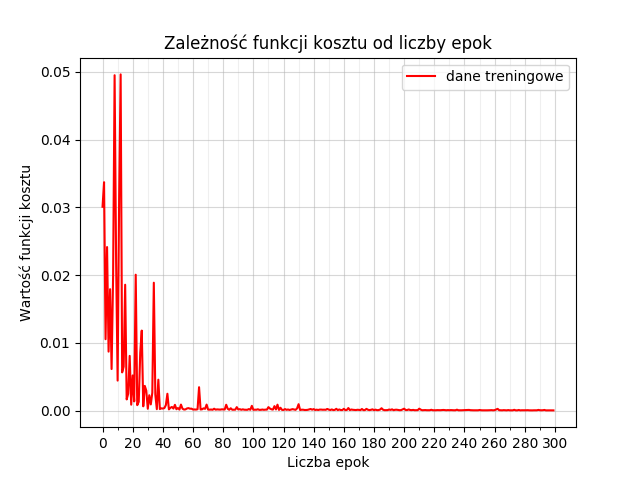
\includegraphics[width=0.7\linewidth]{cost_epoch_150.png}
  \caption{Zależność kosztu od liczby epok dla sieci z 150 neuronami}
\end{figure}

\begin{figure}[h]
  \label{fig:Koszt-liczba-epok-zoom}
  \centering 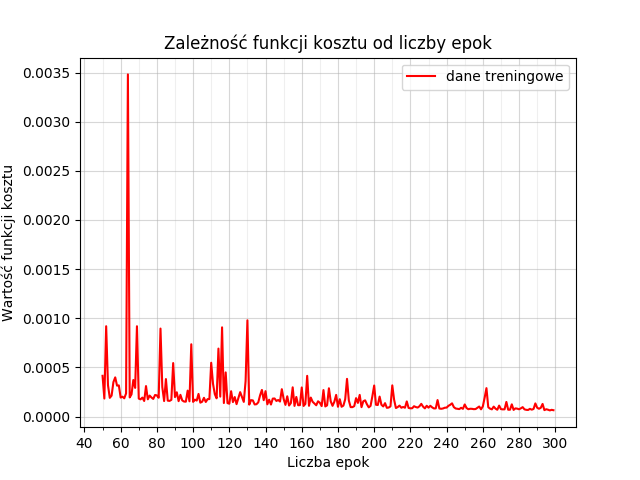
\includegraphics[width=0.7\linewidth]{cost_epoch_150_zoom.png}
  \caption{Zależność kosztu od liczby epok dla sieci z 150 neuronami (ucięte wartości początkowe)}
\end{figure}
 

%- koszt dla roznych wielkosci sieci
%- koszt dla roznej liczby epok 
%- przyklady regulacji z porównaniem MSE


\subsection{Zastosowanie algorytmu OBD}

\begin{figure}[h]
  \label{fig:Koszt-OBD-full}
  \centering 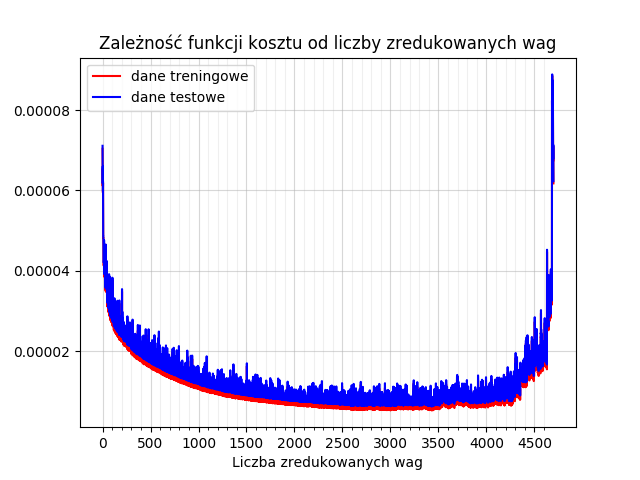
\includegraphics[width=0.7\linewidth]{cost_OBD_full.png}
  \caption{Zależność kosztu od liczby zredukowanych wag - dane testowe i treningowe}
\end{figure}

\subsection{Zastosowanie innych obiektów regulacji}
